\section{Εισαγωγή}
Οι σωροί επιτρέπουν την οργάνωση των δεδομένων με τέτοιο τρόπο έτσι ώστε το μεγαλύτερο στοιχείο να είναι συνεχώς προσπελάσιμο σε σταθερό χρόνο. Η δε λειτουργίες της εισαγωγής νέων τιμών στη δομή και της διαγραφή της μεγαλύτερης τιμής πραγματοποιούνται ταχύτατα. Σε αυτό το εργαστήριο θα παρουσιαστεί η υλοποίηση ενός σωρού μεγίστων και ο σχετικός με τη δομή αυτή αλγόριθμος ταξινόμησης, heapsort. Επιπλέον, θα παρουσιαστεί η δομή std::priority\_queue που υλοποιεί στην STL της C++ τους σωρούς μεγίστων και ελαχίστων. Ο κώδικας όλων των παραδειγμάτων βρίσκεται στο \href{https://github.com/chgogos/ceteiep_dsa}{https://github.com/chgogos/ceteiep\_dsa}.

\section{Σωροί}
Ο σωρός είναι μια μερικά ταξινομημένη δομή δεδομένων. Υπάρχουν δύο βασικά είδη σωρών: ο σωρός μεγίστων (MAXHEAP) και ο σωρός ελαχίστων (MINHEAP). Οι ιδιότητες των σωρών που θα περιγραφούν στη συνέχεια αφορούν τους σωρούς μεγίστων αλλά αντίστοιχες ιδιότητες ισχύουν και για τους σωρούς ελαχίστων. Ειδικότερα, ένας σωρός μεγίστων υποστηρίζει ταχύτατα τις ακόλουθες λειτουργίες:
\begin{itemize}[noitemsep]
\item Εύρεση του στοιχείου με τη μεγαλύτερη τιμή κλειδιού.
\item Διαγραφή του στοιχείου με τη μεγαλύτερη τιμή κλειδιού.
\item Εισαγωγή νέου κλειδιού στη δομή.
\end{itemize}

Ένας σωρός μπορεί να θεωρηθεί ως ένα δυαδικό δένδρο για το οποίο ισχύουν οι ακόλουθοι δύο περιορισμοί:
\begin{itemize}[noitemsep]
\item	Πληρότητα: το δυαδικό δένδρο είναι συμπληρωμένο, δηλαδή όλα τα επίπεδά του είναι πλήρως συμπληρωμένα εκτός πιθανά από το τελευταίο (χαμηλότερο) επίπεδο στο οποίο μπορούν να λείπουν μόνο κάποια από τα δεξιότερα φύλλα.
\item	Κυριαρχία γονέα: το κλειδί σε κάθε κορυφή είναι μεγαλύτερο ή ίσο από τα κλειδιά των παιδιών (σε MAXHEAP).
\end{itemize}

Ένας σωρός μπορεί να υλοποιηθεί με ένα πίνακα καταγράφοντας στον πίνακα στη σειρά τα στοιχεία του δυαδικού δένδρου από αριστερά προς τα δεξιά και από πάνω προς τα κάτω (σχήμα \ref{fig:heap2}). Μερικές σημαντικές ιδιότητες οι οποίες προκύπτουν εφόσον τηρηθεί ο παραπάνω τρόπος αντιστοίχισης των στοιχείων του δένδρου στα στοιχεία του  πίνακα είναι οι ακόλουθες:
\begin{itemize}[noitemsep]
\item	Στον πίνακα, τα κελιά γονείς βρίσκονται στις πρώτες $\lfloor{\frac{n}{2}}\rfloor$ θέσεις ενώ τα φύλλα καταλαμβάνουν τις υπόλοιπες θέσεις. 
\item	Στον πίνακα, τα παιδιά για κάθε κλειδί στις θέσεις $i$ από 1 μέχρι και $\lfloor{\frac{n}{2}}\rfloor$ βρίσκονται στις θέσεις $2*i$ και $2*i + 1$.
\item	Στον πίνακα, ο γονέας για κάθε κλειδί στις θέσεις $i$ από 2 μέχρι και $n$ βρίσκεται στη θέση $\lfloor{\frac{i}{2}}\rfloor$.
\end{itemize}


\begin{figure}[ht]
\centering
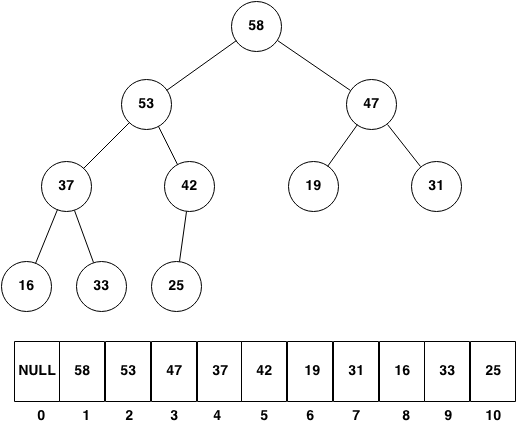
\includegraphics[width=100mm]{heap2.png}
\caption{Αναπαράσταση ενός σωρού μεγίστων ως πίνακα}
\label{fig:heap2}
\end{figure}

Για το παράδειγμα του σχήματος ισχύουν τα ακόλουθα:
\begin{itemize}[noitemsep]
\item Οι κόμβοι που είναι γονείς (έχουν τουλάχιστον ένα παιδί) βρίσκονται στις θέσεις από 1 μέχρι και 5.
\item Οι κόμβοι που είναι φύλλα βρίσκονται στις θέσεις από 6 μέχρι και 10.
\item Ο γονέας στη θέση 1 (η τιμή 58) έχει παιδιά στις θέσεις $2*1=2$ (τιμή 53) και $2*1+1=3$ (τιμή 57).
\item Ο γονέας στη θέση 2 (η τιμή 53) έχει παιδιά στις θέσεις $2*2=4$ (τιμή 37) και $2*2+1=5$ (τιμή 42).
\item Ο γονέας στη θέση 3 (η τιμή 47) έχει παιδιά στις θέσεις $2*3=6$ (τιμή 19) και $2*3+1=7$ (τιμή 31).
\item Ο γονέας στη θέση 4 (η τιμή 37) έχει παιδιά στις θέσεις $2*4=8$ (τιμή 16) και $2*4+1=9$ (τιμή 33).
\item Ο γονέας στη θέση 5 (η τιμή 42) έχει παιδιά στις θέσεις $2*5=10$ (τιμή 25).
\item Ο κόμβος παιδί στη θέση 2 (η τιμή 53) έχει γονέα στη θέση $\lfloor{\frac{2}{2}}\rfloor=1$ (τιμή 58).
\item Ο κόμβος παιδί στη θέση 3 (η τιμή 47) έχει γονέα στη θέση $\lfloor{\frac{3}{2}}\rfloor=1$ (τιμή 58).
\item Ο κόμβος παιδί στη θέση 4 (η τιμή 37) έχει γονέα στη θέση $\lfloor{\frac{4}{2}}\rfloor=2$ (τιμή 53).
\item Ο κόμβος παιδί στη θέση 5 (η τιμή 42) έχει γονέα στη θέση $\lfloor{\frac{5}{2}}\rfloor=2$ (τιμή 53).
\item Ο κόμβος παιδί στη θέση 6 (η τιμή 19) έχει γονέα στη θέση $\lfloor{\frac{6}{2}}\rfloor=3$ (τιμή 47).
\item Ο κόμβος παιδί στη θέση 7 (η τιμή 31) έχει γονέα στη θέση $\lfloor{\frac{7}{2}}\rfloor=3$ (τιμή 47).
\item Ο κόμβος παιδί στη θέση 8 (η τιμή 16) έχει γονέα στη θέση $\lfloor{\frac{8}{2}}\rfloor=4$ (τιμή 37).
\item Ο κόμβος παιδί στη θέση 9 (η τιμή 33) έχει γονέα στη θέση $\lfloor{\frac{9}{2}}\rfloor=4$ (τιμή 37).
\item Ο κόμβος παιδί στη θέση 10 (η τιμή 25) έχει γονέα στη θέση $\lfloor{\frac{10}{2}}\rfloor=5$ (τιμή 42).
\end{itemize}

\section{Υλοποίηση ενός σωρού}
Στη συνέχεια παρουσιάζεται η υλοποίηση ενός σωρού μεγίστων που περιέχει ακέραιες τιμές-κλειδιά.

\lstinputlisting[caption = Σωρός μεγίστων με κλειδιά ακέραιες τιμές (max\_heap.cpp)]{lab06/max_heap.cpp}

\subsubsection*{Η συνάρτηση λήψης της μεγαλύτερης τιμής (top)}
Καθώς η μεγαλύτερη τιμή βρίσκεται πάντα στη θέση 1 του πίνακα που διατηρεί τα δεδομένα του σωρού η συνάρτηση top απλά επιστρέφει την τιμή αυτή.
\subsubsection*{Η συνάρτηση εξαγωγής της μεγαλύτερης τιμής (pop)}
Η εξαγωγή της μεγαλύτερη τιμής γίνεται ως εξής. Το στοιχείο που βρίσκεται στην κορυφή του σωρού αντιμετατίθεται με το τελειταίο στοιχείο του σωρού. Στην συνέχεια το στοιχείο που έχει βρεθεί στην κορυφή του σωρού κατεβαίνει προς τα κάτω αν έχει παιδί που είναι μεγαλύτερό του πραγματοποιώντας αντιμετάθεση με το μεγαλύτερο στοιχείο από τα παιδιά του. Η διαδικασία επαναλαμβάνεται για τη νέα θέση του στοιχείου που αρχικά είχε μεταφερθεί στη κορυφή και μέχρι να ισχύσει ότι είναι μεγαλύτερο και από τα δύο παιδιά του.
\subsubsection*{Η συνάρτηση εισαγωγής νέας τιμής (push)}
Η εισαγωγή ενός στοιχείου γίνεται ως φύλλο στη πρώτη διαθέσιμη θέση από πάνω προς τα κάτω και από δεξιά προς τα αριστερά. Το στοιχείο αυτό συγκρίνεται με το γονέα του και αν είναι μεγαλύτερο αντιμετατίθεται με αυτόν. Η διαδικασία συνεχίζεται μέχρι είτε να βρεθεί το νέο στοιχείο στην κορυφή είτε να ισχύει η κυριαρχία γονέα.

Ο ακόλουθος κώδικας χρησιμοποιεί τη συνάρτηση heap\_bottom\_up και μέσω αυτής τη συνάρτηση heapify προκειμένου να μετασχηματίσει έναν πίνακα ακεραίων σε σωρό μεγίστων. 
\lstinputlisting[caption = Δημιουργία σωρού από πίνακα με heapify (heap1.cpp)]{lab06/heap1.cpp}

\lstinputlisting[style=DOS]{lab06/heap1.out}

Ο ακόλουθος κώδικας δημιουργεί σταδιακά έναν σωρό εισάγοντας δέκα τιμές με τη συνάρτηση push. Στη συνέχεια πραγματοποιούνται εξαγωγές τιμών με τη συνάρτηση pop μέχρι ο σωρός να αδειάσει.

\lstinputlisting[caption = Δημιουργία σωρού με εισαγωγές τιμών και εν συνεχεία άδειασμα του σωρού με διαδοχικές διαγραφές της μέγιστης τιμής (heap2.cpp)]{lab06/heap2.cpp}

\lstinputlisting[style=DOS]{lab06/heap2.out}


\section{Ταξινόμηση Heapsort}
Ο αλγόριθμος Heapsort προτάθηκε από τον J.W.J.Williams το 1964 και αποτελείται από 2 στάδια:
\begin{itemize}[noitemsep]
\item Δημιουργία σωρού με τα n στοιχεία ενός πίνακα τα στοιχεία του οποίου ζητείται να ταξινομηθούν. 
\item Εφαρμογή της διαγραφής της ρίζας n -1 φορές.
\end{itemize}
Το αποτέλεσμα είναι ότι τα στοιχεία αφαιρούνται από το σωρό σε φθίνουσα σειρά. Καθώς κατά την αφαίρεσή του κάθε στοιχείου, αυτό τοποθετείται στο τέλος του σωρού, τελικά ο σωρός περιέχει τα αρχικά δεδομένα σε αύξουσα σειρά. Στη συνέχεια παρουσιάζεται η υλοποίηση του αλγορίθμου HeapSort. Επιπλέον ο κώδικας ταξινομεί πίνακες μεγέθους 10.000, 20.000, 40.000 80.000 και 100.000 που περιέχουν τυχαίες ακέραιες τιμές και πραγματοποιείται σύγκριση με τους χρόνους εκτέλεσης που επιτυγχάνει η std::sort.

\lstinputlisting[caption = Ο αλγόριθμος heapsort (heapsort.cpp)]{lab06/heapsort.cpp}

\lstinputlisting[style=DOS]{lab06/heapsort.out}


\section{Η δομή priority\_queue της STL}
Η STL της C++ περιέχει υλοποίηση της δομής std::priority\_queue (ουρά προτεραιότητας) η οποία είναι ένας σωρός μεγίστων. Κάθε στοιχείο που εισέρχεται  στην ουρά προτεραιότητας έχει μια προτεραιότητα που συνδέεται με αυτό και το στοιχείο με τη μεγαλύτερη προτεραιότητα βρίσκεται πάντα στην αρχή της ουράς. Οι κυριότερες λειτουργίες που υποστηρίζονται από την std::priority\_queue είναι οι ακόλουθες:
\begin{itemize}[noitemsep]
\item push: εισαγωγή ενός στοιχείου στη δομή.
\item top: επιστροφή χωρίς εξαγωγή του στοιχείου με τη μεγαλύτερη προτεραιότητα.
\item pop: απώθηση του στοιχείου με τη μεγαλύτερη προτεραιότητα.
\item size: πλήθος των στοιχείων που υπάρχουν στη δομή.
\item empty: επιστρέφει true αν η δομή είναι άδεια αλλιώς επιστρέφει false.
\end{itemize}
Ένα παράδειγμα χρήσης της std::priority\_queue ως σωρού μεγίστων αλλά και ως σωρού ελαχίστων παρουσιάζεται στη συνέχεια.

\lstinputlisting[caption = Παράδειγμα με priority\_queue της STL (stl\_priority\_queue.cpp)]{lab06/stl_priority_queue.cpp}

\lstinputlisting[style=DOS]{lab06/stl_priority_queue.out}


\section{Παραδείγματα}
\subsection{Παράδειγμα 1}
Χρησιμοποιώντας τον κώδικα 1, να γραφεί κώδικας που να εισάγει 50.000 τυχαίες ακέραιες τιμές σε έναν σωρό μεγίστων με τη συνάρτηση heap\_bottom\_up καθώς και με τη συνάρτηση push. Χρονομετρείστε τον κώδικα και στις δύο περιπτώσεις δημιουργίας του σωρού.

\subsection{Παράδειγμα 2}
Διάμεσος ενός δείγματος Ν παρατηρήσεων οι οποίες έχουν διαταχθεί σε αύξουσα σειρά ορίζεται ως η μεσαία παρατήρηση, όταν το Ν είναι περιττός αριθμός, ή ο μέσος όρος (ημιάθροισμα) των δύο μεσαίων παρατηρήσεων όταν το Ν είναι άρτιος αριθμός. 
Έστω ότι για διάφορες τιμές που παράγονται με κάποιον τρόπο ζητείται ο υπολογισμός της διάμεσης  τιμής καθώς παράγεται κάθε νέα τιμή και για όλες τις τιμές που έχουν προηγηθεί μαζί με την τρέχουσα τιμή όπως φαίνεται στο επόμενο παράδειγμα:\\ 
5  $\Rightarrow$  διάμεσος 5\\
5, 7 $\Rightarrow$ διάμεσος 6\\
5, 7, 13 $\Rightarrow$ διάμεσος 7\\
5, 7, 13, 12 $\Rightarrow$ 5, 7, 12, 13 $\Rightarrow$ διάμεσος 9.5\\
5, 7, 13, 12, 2 $\Rightarrow$ 2, 5, 7, 12, 13 $\Rightarrow$ διάμεσος 7

\lstinputlisting[caption = Υπολογισμός διαμέσου σε μια ροή τιμών (lab06\_ex1.cpp)]{lab06/lab06_ex1.cpp}

\lstinputlisting[style=DOS]{lab06/lab06_ex1.out}

\subsection{Παράδειγμα 3}

\section{Ασκήσεις}
\begin{enumerate}
\item Να υλοποιηθεί ο σωρός μεγίστων που παρουσιάστηκε στον κώδικα 1 ως κλάση. Προσθέστε εξαιρέσεις έτσι ώστε να χειρίζονται περιπτώσεις όπως όταν ο σωρός είναι άδειος και ζητείται εξαγωγή της μεγαλύτερης τιμής ή όταν ο σωρός είναι γεμάτος και επιχειρείται εισαγωγή νέας τιμής.
\item Να γραφεί συνάρτηση που να δέχεται ως παράμετρο έναν πίνακα ακεραίων και έναν ακέραιο αριθμό κ και να επιστρέφει το κ-οστό μεγαλύτερο στοιχείο του πίνακα. 
%\item b
%\item d
\end{enumerate}

\begin{thebibliography}{9}
\bibitem{cppexceptions}
Geeks for Geeks, Priority Queue in C++ Standard Template Library (STL), \href{http://www.geeksforgeeks.org/priority-queue-in-cpp-stl/}{http://www.geeksforgeeks.org/priority-queue-in-cpp-stl/}
\end{thebibliography}

